\section{The authors' camera: Sun track and pose}

The Sun found in every logged frame (brightest saturated plateau within 25$^\circ$ of the ring of the Sun's zenith angle under the declared zenith pointing; quarter-resolution decode, 31-px window) as a camera-frame ray through the nominal fisheye model of P042, fitted against the sidecars' Sun vectors with P044's trimmed Kabsch. The declared pointing is the identity rotation; its residual is what the P083/P084/P090 ray maps carried.

{\tiny\setlength{\tabcolsep}{3pt}
\begin{longtable}{llllllllll}
\toprule
Days & Frames & Detections & Inliers & Span (h) & Declared median / p90 ($^\circ$) & Fitted median / p90 ($^\circ$) & Roll / pitch / yaw ($^\circ$) & Yaw by azimuth difference, median (IQR) & Status \\
\midrule
\endhead
all & 273 & 269 & 267 & 71.9 & 106.80 / 126.29 & 9.08 / 15.98 & -4.3 / 12.1 / 161.9 & 210.1 (26.1) & insufficient \\
2026-10-18 & 120 & 116 & 116 & 1.0 & 123.21 / 128.64 & 5.93 / 10.73 & not identifiable (arc $<$ 3 h) & 221.3 (7.2) & insufficient \\
2026-10-19 & 120 & 120 & 118 & 1.0 & 98.62 / 108.31 & 9.44 / 16.19 & not identifiable (arc $<$ 3 h) & 201.8 (15.2) & insufficient \\
2026-10-21 & 33 & 33 & 26 & 1.7 & 69.14 / 100.81 & 3.25 / 8.19 & not identifiable (arc $<$ 3 h) & 185.0 (12.3) & insufficient \\
\bottomrule
\end{longtable}}

Status rule (P044): inliers $\geq$ 15, span $\geq$ 3.0 h, median $\leq$ 1.0$^\circ$, p90 $\leq$ 2.0$^\circ$ on the inliers. The nominal model is the datasheet fisheye (f = 2540.7 px, no measured distortion), and the detector takes the centre of a saturated plateau that can span 40$^\circ$ of sky, so a residual well above the Eye2Sky 0.1$^\circ$ says 'intrinsics and detector' as much as 'pose'; the yaw is the robust part (it only needs the Sun's azimuth in the picture).

\subsection{Focal scale}

The fit with the nominal focal length scaled. The residual falls slowly as the focal grows while the inferred axis tilt grows with it: focal and tilt are degenerate under this detector, so the scan is a diagnostic and the nominal focal is kept; a checkerboard calibration (P031) is what resolves it.

{\scriptsize\setlength{\tabcolsep}{3pt}
\begin{longtable}{llllll}
\toprule
Focal $\times$ & n & Median ($^\circ$) & p90 ($^\circ$) & Yaw ($^\circ$) & Axis elevation ($^\circ$) \\
\midrule
\endhead
0.8 & 269 & 11.04 & 18.59 & 161.0 & 86.5 \\
0.9 & 269 & 9.98 & 16.89 & 161.7 & 82.2 \\
1.0 & 269 & 9.08 & 15.98 & 161.9 & 77.1 \\
1.1 & 269 & 8.62 & 14.89 & 162.0 & 72.9 \\
1.2 & 269 & 8.19 & 14.24 & 161.8 & 69.3 \\
1.3 & 269 & 7.88 & 13.63 & 161.6 & 66.2 \\
1.5 & 269 & 7.29 & 12.75 & 160.9 & 61.2 \\
\bottomrule
\end{longtable}}

\begin{figure}[h]
\centering
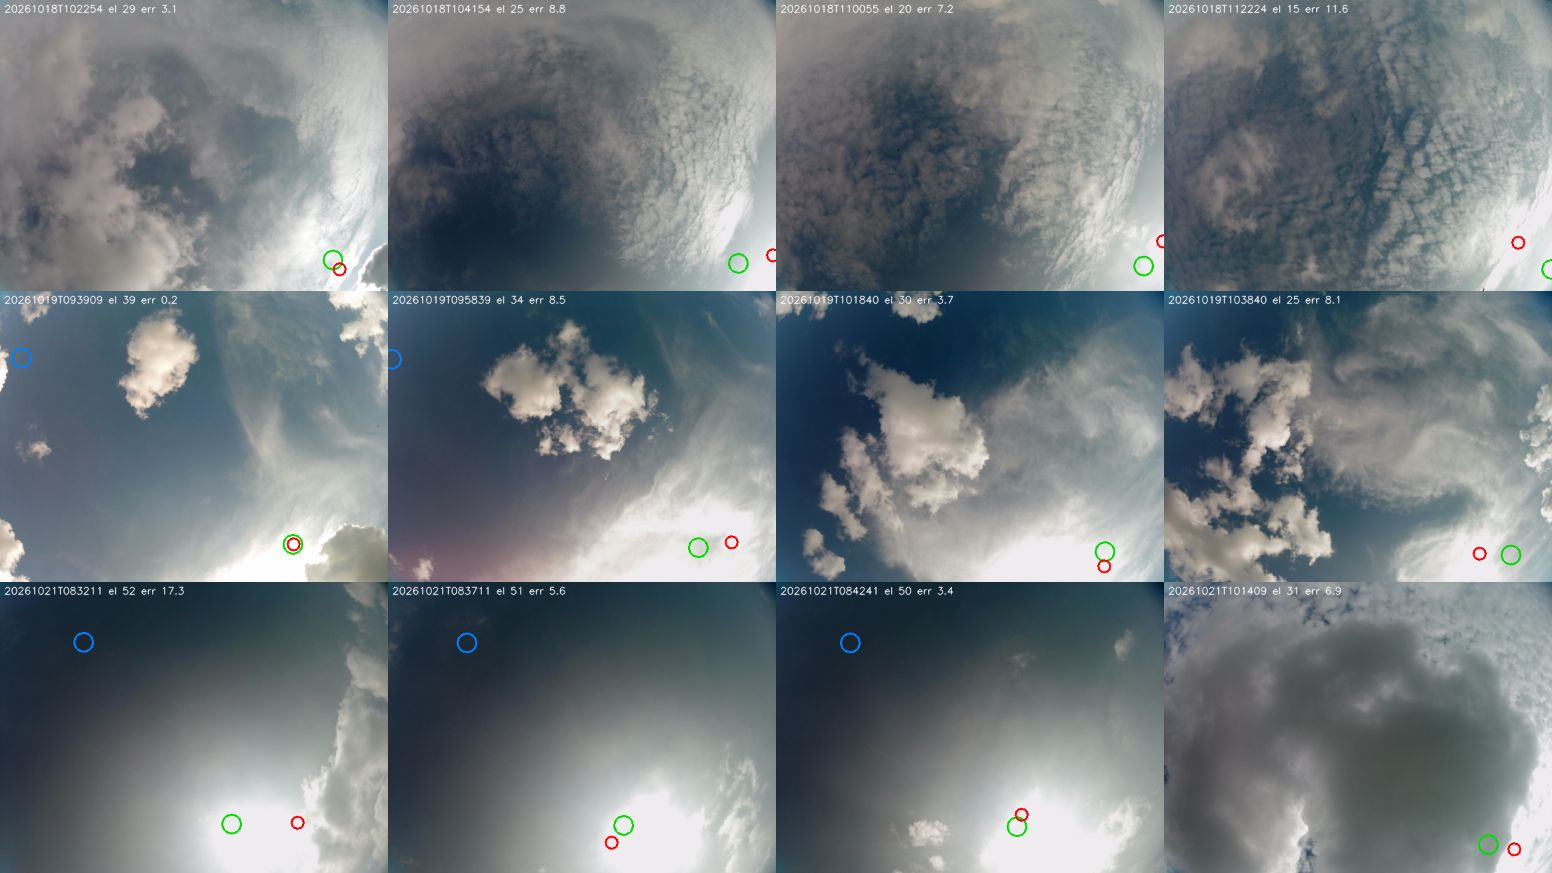
\includegraphics[width=0.9\linewidth]{supp/fig/b0268_sun_track.jpg}
\caption{detections against the declared and fitted poses}
\end{figure}

Twelve frames, four per day: red = detected plateau, blue = the Sun under the declared identity pose (off the glare in every frame), green = under the fitted pose.

Rows in \texttt{data/b0268\_sun\_track.parquet}; the pose record \texttt{BLR01\_b0268\_nominal} in \texttt{configs/camera\_poses.yaml} (nothing reads it yet: the P083/P084 ray maps and the locked-day evaluation used the declared identity pose and stay as reported).

